\section{Implementation}
\subsection{Socket programming}
\begin{frame}{Bad performance with interrupts}{}
	\begin{alertblock}{Standard socket programming is interrupt based}
		Every hardware and software (syscall) interrupt induces a context switch
		($\approx$100~ns)\\
		\begin{ergo}
			High packet loss ($>10^{-5} \Rightarrow $ loose $>$100 Mio. events)
		\end{ergo}
	\end{alertblock}
	
	\begin{ergo}
		No problem for web apps but I cannot use kernel sockets!
	\end{ergo}
\end{frame}

\begin{frame}{Solution: pf\_ring DNA - new type of network socket}{}
	\begin{center} 
		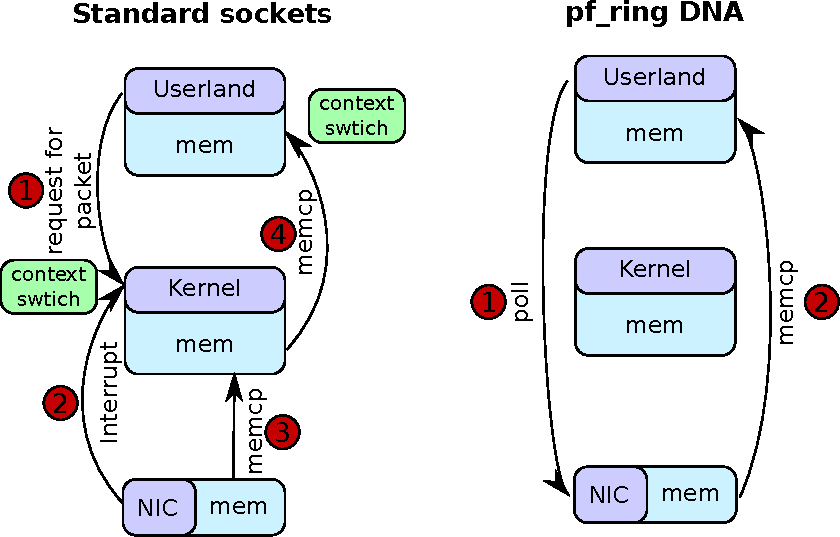
\includegraphics[height=4.5cm]{kernel-socket-vs-pf_ring}
	\end{center}
\end{frame}

\begin{frame}{pf\_ring DNA}{}
	\begin{block}{Special socket: pf\_ring DNA by ntop (open source)}
		\begin{itemize}
		  \item Polling the NIC memory directly (avoids system calls)
		  \item Only $\approx$40\% CPU @ full speed 10~G receiving 1~kB packets
		  \item No packet loss at all
		\end{itemize}
	\end{block}
	
	\begin{alertblock}{pf\_ring does not yet support any protocol}
		\begin{itemize}
		  \item Every byte has to be moved by the user
		  \item I had to implement Ethernet, IP, UDP, ARP and IGMP
		\end{itemize}
	\end{alertblock}
	
	\begin{ergo}
		270~kHz Eventbuilding rate with <5 virtual cores \\
		$\Rightarrow$ >19 cores left for L1 and L2 trigger
	\end{ergo}
\end{frame}



\subsection{Parallel programming}
\begin{frame}{Same problem with Mutex/Semaphore}{}
	\begin{block}{Bad performance with Mutexes/Semaphores}
		\begin{ergo}
			Implemented lockless queues based on consumer-producer communications
		\end{ergo}
	\end{block}
	\begin{center} 
		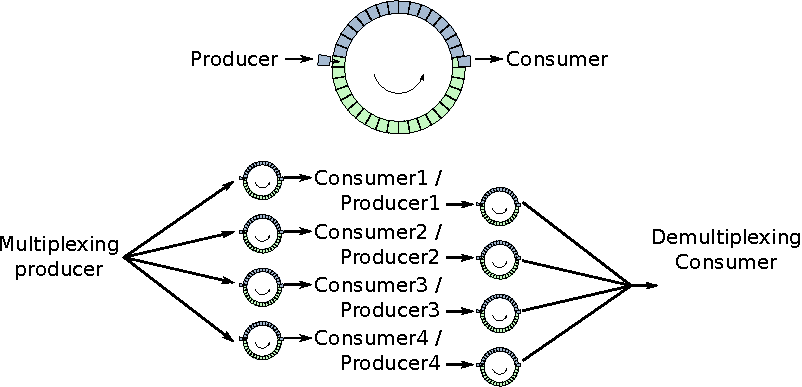
\includegraphics[height=4.5cm]{consumer-producer-queue}	
	\end{center}
\end{frame}
